\documentclass{article}
\usepackage[utf8]{inputenc}
\usepackage[margin=1in]{geometry}
\setlength{\parindent}{0em}
\setlength{\parskip}{0.5em}
\usepackage[backend=biber,sorting=none]{biblatex}
\usepackage{amsmath, amsthm, graphicx, mathtools, amsfonts, xurl, siunitx, makecell, caption, gensymb, chemformula, float, etoolbox, titlesec}
\titleformat{\subsection}[runin]
{\normalfont\bfseries}{\thesubsection}{1em}{}
\DeclareMathOperator{\tr}{tr}
\AtBeginEnvironment{bmatrix}{\setlength{\arraycolsep}{8pt}}
\captionsetup[table]{labelfont={bf}, labelsep=period, skip=8pt}
\captionsetup[figure]{labelfont={bf}, labelsep=period}
\renewcommand\vec{\mathbf}
\addbibresource{Lake.bib}

\title{2-D modeling of cyanobacterial blooms over time}
\author{Chu Chen}
\date{May 1, 2019}

\begin{document}

\maketitle

\textbf{Abstract} \quad\space Cyanobacterial blooms are worldwide environmental issues associated with eutrophication of water bodies. In this study, I built up a 2-D advection-reaction-diffusion model to quantify how the density of cyanobacteria, the density of zooplankton, and the concentration of dissolved phosphorus evolve. By applying this model to an ideal river with laminar flow, I explained why cyanobacteria density near the bank sometimes appears higher compared to the center of slow-flowing eutrophic rivers. This modeling framework may be refined to serve as a tool to forecast cyanobacterial blooms and to study the effectiveness of different controlling measures.

\textbf{Keywords} \quad cyanobacterial bloom \quad eutrophication \quad advection-reaction-diffusion system
\bigskip
\hrule

\section*{Backgrounds}
Nowadays, cyanobacterial blooms are worldwide environmental issues posing great threats to ecosystems and human society. Fertilizer runoff and municipal sewage, among other sources, supply water bodies with a large amount of phosphorus and/or nitrogen (eutrophication), favoring cyanobacteria outgrowth. Presence of a high density of cyanobacteria may alter the physicochemical properties of water bodies (like turbidity, pH, and dissolved oxygen level), which can hugely impact aquatic lives. Some species of cyanobacteria produce 2-methylisoborneol and geosmin, which inflict an earthy taste on fish and drinking water. Certain strains of cyanobacteria may even produce cyanotoxins that are poisonous to human beings and other animals \cite{GrazerSize}.

\begin{figure}[H]
    \centering
    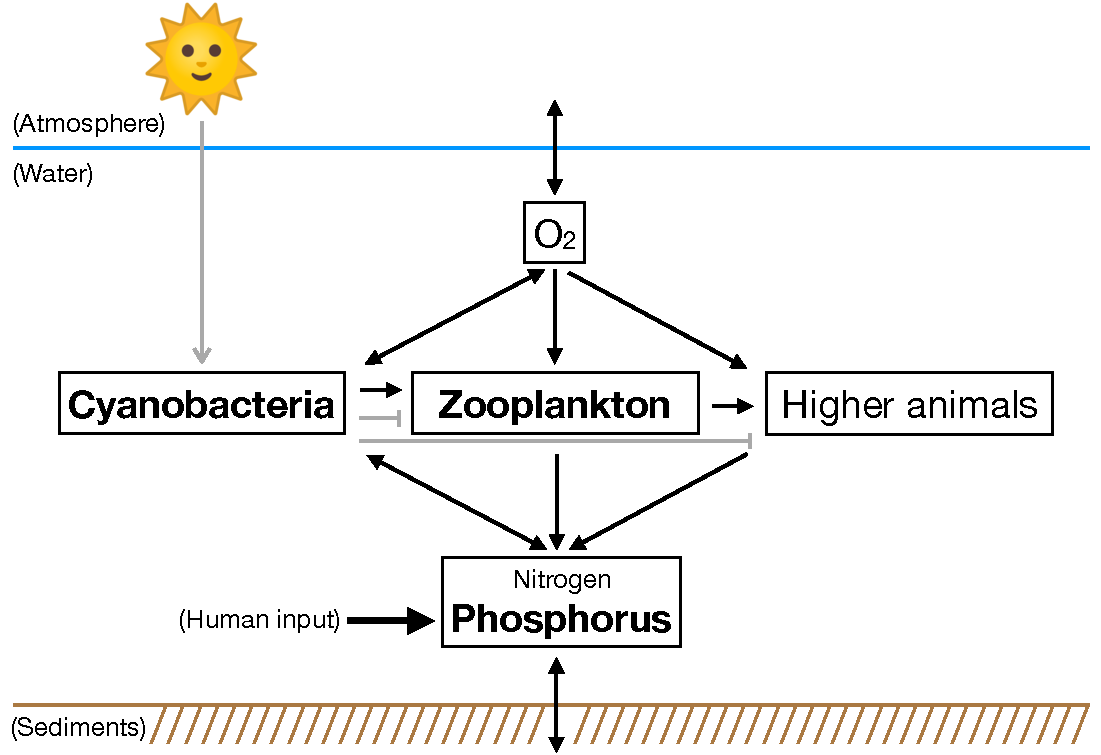
\includegraphics[width=0.55\textwidth]{SpeciesInteraction.pdf}
    \caption{\textbf{A diagram of main interactions and substance flow between key components of an aquatic ecosystem.} Cyanobacteria contribute to dissolved nutrients by decomposition of dead cyanobacteria, excretion of live cyanobacteria, and the nitrogen-fixing activity of certain cyanobacteria species \cite{LimitingFactor}. Decomposition consumes dissolved oxygen \cite{GrazerSize}. In this study, we will focus on the dynamics of cyanobacteria, zooplankton, and the dissolved limiting nutrient.}
    \label{AquaticEcosystem}
\end{figure}

A large number of experimental and modeling studies have been performed on different aspects of the mechanics of cyanobacterial blooms. However, most of the modeling studies were based on ordinary differential equations (ODEs) of closed systems developing over time \cite{SteeleHenderson, DumitranVuta}. Very few studies have accounted for fluid dynamics and spatial heterogeneity of realistic water bodies \cite{2D-B, ZhaoTianWei}.

In this study, I will build up a 2-D partial differential equation (PDE) model to quantify how the density of cyanobacteria, the density of zooplankton, and the concentration of the dissolved limiting nutrient (\textbf{Figure \ref{AquaticEcosystem}}) evolve in the presence of advection and diffusion. By applying this model to a river with laminar flow and using finite-difference numerical simulation, I will provide an explanation of why cyanobacteria density near the bank is sometimes higher compared to the center of slow-flowing eutrophic streams.

\section*{Models \& methods}
\subsection*{A river with laminar flow (toy model)}
Let us consider a river which is straight with a rectangular channel, whose width, slope, and discharge are all constant (\textbf{Figure \ref{ToyRiverVelocityProfile}}).

\begin{figure}[h]
    \centering
    \captionsetup{justification=centering}
    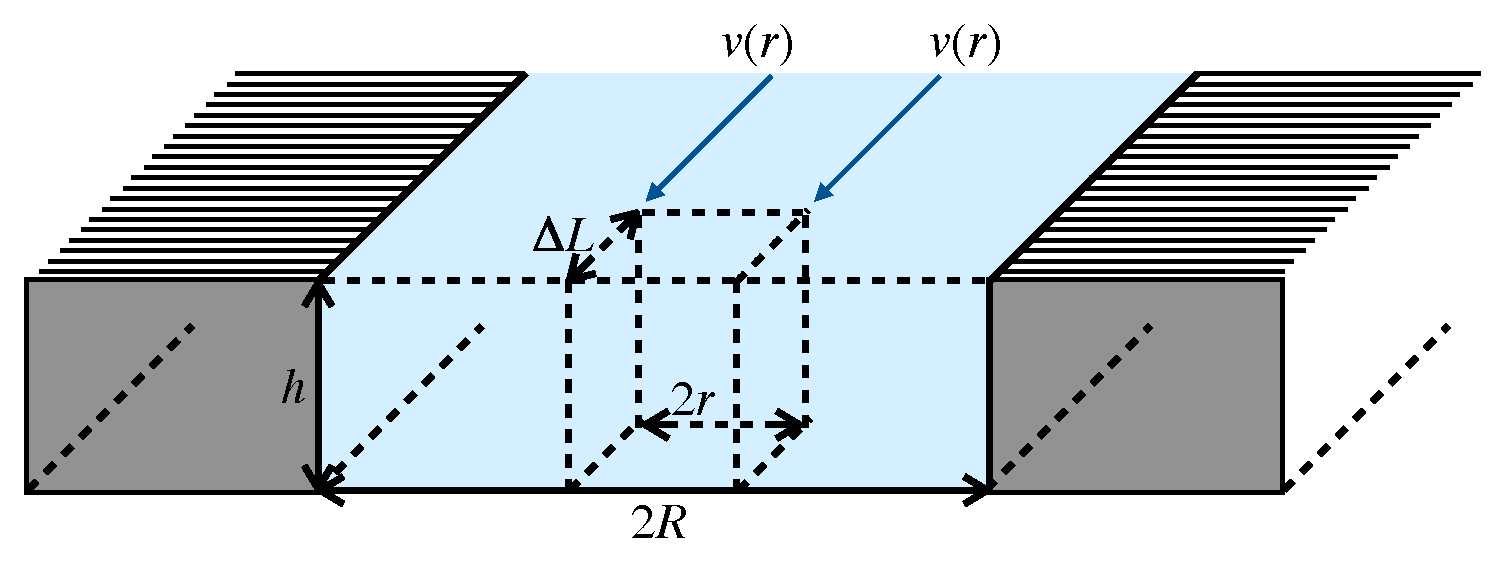
\includegraphics[width=0.5\textwidth]{ToyRiverDiagram.pdf}
    \caption{\textbf{A diagram of the river in the toy model.}}
    \label{ToyRiverVelocityProfile}
\end{figure}

Under the condition that flow velocity at a certain point is a function of only the distance $r$ of that point to the center line of the river (\textit{i.e.}, changes across the width of the river but not along its length or depth)
\begin{equation*}
    |\vec{v}| = v(r),
\end{equation*}
the depth $h$ must also not change along the length of the river according to the principle of mass conservation. This condition also implies that the shear stress of water (Newtonian fluid with viscosity $\mu$) is in balance with other forces, including the downstream component of gravity and friction against the bed. The resultant of the gravity component and friction is proportional to the volume (here we designate the coefficient as $B$). We can write down the force balance equation for a segment of river with width $2r$ (symmetric about the center line of the river) and length $\Delta L$ as
\begin{equation*}
    2\mu v'(r) h \Delta L + 2r h \Delta L B = 0.
\end{equation*}
Therefore,
\begin{equation*}
    v(r) = -\frac{B}{2\mu}r^2 + C.
\end{equation*}
This indicates that the velocity profile features a parabola, with maximum velocity taken along the center line of the river $v_{\max} = v(0) = C$. Let us designate the width of the river as $2R$ $(0 \leq r \leq R)$. Since the flow velocity along the river bank is 0, we have
\begin{equation*}
    v(R) = -\frac{B}{2\mu}R^2 + v_{\max} = 0,
\end{equation*}
or $v_{\max} =  BR^2/(2\mu)$. Substitution of variables yields
\begin{equation}
    v(r) = v_{\max}(1 - \frac{r^2}{R^2}).
    \label{v-r}
\end{equation}

\subsection*{Turnover-flux equations}
In this preliminary study on 2-D models, the variability of temperature or sunlight conditions over space or time is not considered. The only environmental factor that affects the growth rate of cyanobacteria is nutrient availability. Here, let us assume that phosphorus is the rate-limiting factor \cite{LimitingFactor}. For simplification, dissolved phosphorus in the environment is treated as a single pool (no compartmentation in particulates). Organic phosphorus in remains and excretions immediately enters this pool and becomes available for assimilation (no necessity of decomposition into phosphate). Exchange with the bottom sedimentation layer is ignored. In addition, only two trophic levels (cyanobacteria and zooplankton) are modeled. The Lotka-Volterra equations (with Holling's Type II functional response, although some filter feeders reportedly feature Type I functional response) are modified to include flux terms \cite{DumitranVuta, Holling, FilterFeeder, PlanktonSystems}. Since little evidence supports the existence of taxis towards cyanobacterial food source for zooplankton as to our knowledge, no such term is incorporated. The resulting governing equations for the density of cyanobacteria $B$, the density of zooplankton $Z$, and the concentration of dissolved phosphorus $P$ are
\begin{alignat}{3}
    &\frac{\partial B}{\partial t} &&= \beta\frac{P}{P + \kappa_P}B - \zeta\frac{B}{B + \kappa_B}Z && - \vec{v} \cdot \nabla B, \label{B-t}\\
    &\frac{\partial Z}{\partial t} &&= (\epsilon\zeta\frac{B}{B + \kappa_B} - \theta) Z &&+ (D_Z\nabla - \vec{v}) \cdot \nabla Z, \label{Z-t}\\
    &\frac{\partial P}{\partial t} &&= -\omega(\frac{\partial B}{\partial t} + \frac{\partial Z}{\partial t}) &&+ (D_P\nabla - \vec{v}) \cdot \nabla P \label{P-t}.
\end{alignat}
Although pilus-like structures that may facilitate mobility are observed on certain strains of bloom-forming cyanobacteria \cite{MaPilus, Mw}, the fact that they typically clump into colonies during a bloom justifies the omission of a diffusion term in equation (\ref{B-t}) above. The meanings and values of parameters in the equations above are listed in \textbf{Table \ref{Parameters}}.

\begin{table}[H]
    \renewcommand{\arraystretch}{2}
    \caption{\textbf{Constant parameters in the turnover-flux equations.} $\beta$, $\omega$, and $\kappa_P$ are determined for \textit{Microcystis} sp. An assimilation efficiency $\epsilon$ of 0.7 is a consensus in modeling studies. Self-diffusion coefficient of \ch{H2PO4^{-}} at infinite dilution and $18 \degree\text{C}$ is used as $D_P$. The effective diffusion coefficient of \textit{Daphnia magna} (a species of water flea) adults at 21 - $23 \degree \text{C}$ is used as $D_Z$. $\zeta$ is the average of measured maximum ingestion rates of \textit{D. magna} at $20 \degree\text{C}$ listed in the citation. Compared to small-bodied zooplankton, large generalist grazers like \textit{Daphnia} are more effective at controlling cyanobacteria \cite{GrazerSize}. $\theta$ is calculated from an average growth yield $\eta$ of 0.33 concluded in the citation via $\theta = (\epsilon - \eta)\zeta$. $\kappa_B$ is the average half-saturation constant for grazing of Dinoflagellata, Ciliophora, Rotifera, and Sarcomastigophora listed in the citation.}
    \label{Parameters}
    \centering
    \begin{tabular}{c c c c}
        \hline
        Symbol & Parameter & Value & Reference(s) \\
        \hline
        $\beta$ & Maximum cyanobacteria net growth rate & \SI{0.045}{h^{-1}} & \cite{B}\\
        $\zeta$ & Maximum zooplankton ingestion rate & \SI{0.04}{h^{-1}} & \cite{Zeta}\\
        $\epsilon$ & Assimilation efficiency & 0.7 & \cite{Assimilation}\\
        $\omega$ & Phosphorus content in organisms & 0.006 & \cite{MicrocystisPContent}\\
        $\theta$ & \makecell{Death (natural/predation) plus excretion\\and respiration rate of zooplankton} & \SI{0.015}{h^{-1}} & \cite{Zeta}\\
        $\kappa_P$ & \makecell{Phosphorus concentration at which\\cyanobacteria net growth rate reaches $\beta/2$} & \SI{0.015}{mg/L} & \cite{B}\\
        $\kappa_B$ & \makecell{Cyanobacteria density at which\\zooplankton predation reaches $\zeta/2$}& \SI{3}{mg/L} & \cite{KappaBmeta}\\
        $D_Z$ & \makecell{Effective diffusion coefficient of\\zooplankton (correlated random walk)} & \SI{2.17e-6}{m^2/s} & \cite{DZTheory, DZExperiment} \\
        $D_P$ & Diffusion coefficient of dissolved phosphorus & \SI{7.15e-10}{m^2/s} & \cite{DP} \\
        \hline
    \end{tabular}
\end{table}

\subsection*{The numerical simulation algorithm}

The river segment in the toy model (with a width of $m\Delta y$ and a length of $n\Delta x$) is discretized into a 2-D matrix $\vec{A} = (a_{ij}) \in \mathbb{R}^{m \times n}$. It flows from left to right. Each element $a_{ij}$ represents a tile with an area of $\Delta x \cdot \Delta y$ whose center is $d_i = |(i - 1/2)\Delta y - m\Delta y/2|$ away from the center axis of the river and $l_j = (j - 1)\Delta x$ downstream from the starting line (the line crossing the centers of tiles represented by the first column and subject to the Dirichlet boundary condition). Each tile has 3 properties: the density of cyanobacteria $B_{ij}(t)$, the density of zooplankton $Z_{ij}(t)$, and the concentration of dissolved phosphorus $P_{ij}(t)$. Initial conditions are set to be $\vec{a}_{ij}(0) = (B_{ij}(0), Z_{ij}(0), P_{ij}(0)) = (0, 0, 0)$ for all $j > 1$ and $i$. The steady-state matrix is approximated by allowing the system to develop for a duration of time sufficient for the slowest streamlines (ones along the first and last rows) to travel 3 times the length of the river segment. This entire simulation is discretized into time steps of $\Delta t$ and looped through the following the routine:

(i) Reset the Dirichlet boundary condition $\vec{a}_{i1}$;

(ii) Advect via $\vec{a}_{ij}(n\Delta t) \coloneqq ([\hat{j}] - \hat{j} + 1) \cdot \vec{a}_{i[\hat{j}]}((n - 1)\Delta t) + (\hat{j} - [\hat{j}]) \cdot \vec{a}_{i([\hat{j}] + 1)}((n - 1)\Delta t)$, where $\hat{j} \coloneqq j - v(d_i)\Delta t/\Delta x$ and $v(d_i)$ is calculated using equation (\ref{v-r});

(iii) Diffuse in 2-D using the alternating direction implicit method \cite{ADI};

(iv) Develop $\vec{a}_{ij}$ according to \textbf{the turnover equations}:
\begin{align*}
    \frac{d B}{d t} &= \beta\frac{P}{P + \kappa_P}B - \zeta\frac{B}{B + \kappa_B}Z,\\
    \frac{d Z}{d t} &= (\epsilon\zeta\frac{B}{B + \kappa_B} - \theta) Z,\\
    \frac{d P}{d t} &= -\omega(\frac{d B}{d t} + \frac{d Z}{d t}),
\end{align*}
using the Runge-Kutta method (while keeping the total phosphorus level within each tile conserved).

Numerical simulation codes are written in MATLAB\textsuperscript{\tiny\textregistered} and publicly accessible at \url{https://github.com/CreLox/CyanobacteriaBloom}.

\section*{Results}
\subsection*{Linear stability analysis of the turnover equations}
Let us first investigate the turnover equations (ODEs without the diffusion term or the advection term) and examine the fixed points of this time-invariant system using linear stability analysis. It should be noted that as cited in \cite{SteeleHenderson}, fixed points and their stability might behave differently with the presence of the diffusion terms, as well as numerical errors introduced during the simulation.

All fixed points reside on 3 curves in the $(B, Z, P)$ space: $(0, 0, P)$ and $(B, 0, 0)$ represent scenarios where either zooplankton or cyanobacteria die out, with the non-degenerate ones being:
\begin{equation}
    (\frac{\theta}{\epsilon\zeta-\theta}\kappa_B, \frac{\beta\epsilon}{\epsilon\zeta-\theta}\frac{P}{P+\kappa_P}\kappa_B, P). \label{Non-trivialFP}
\end{equation} 
The Jacobian matrix of these autonomous ODEs is
\begin{equation*}
    \vec{J} = \begin{bmatrix}
    \dfrac{\beta P}{P + \kappa_P} - \dfrac{\zeta \kappa_B Z}{(B + \kappa_B)^2} & - \dfrac{\zeta B}{B + \kappa_B} & \dfrac{\beta \kappa_P B}{(P + \kappa_P)^2} \\[1.5em]
    \dfrac{\epsilon \zeta \kappa_B Z}{(B + \kappa_B)^2} & \dfrac{\epsilon \zeta B}{B + \kappa_B} - \theta & 0 \\[1.5em]
    -\dfrac{\omega \beta P}{P + \kappa_P} + \dfrac{\omega (1 - \epsilon) \zeta \kappa_B Z}{(B + \kappa_B)^2} & \dfrac{\omega (1 - \epsilon) \zeta B}{B + \kappa_B} + \omega \theta & -\dfrac{\omega \beta \kappa_P B}{(P + \kappa_P)^2}
    \end{bmatrix}.
\end{equation*}
(i) When evaluated along $(0, 0, P)$, $\vec{J}$ becomes
\begin{equation*}
    \begin{bmatrix}
    \dfrac{\beta P}{P + \kappa_P} & 0 & 0 \\[1.5em]
    0 & - \theta & 0 \\[1.5em]
    -\dfrac{\omega \beta P}{P + \kappa_P} & \omega \theta & 0
    \end{bmatrix},
\end{equation*}
which indicates that $(0, 0, P)$ is not stable since $\beta P/(P + \kappa_P) > 0$ (note that this system will never reach $(0, 0, 0)$ if initially not all of $B, P, Z$ are 0, given that the total phosphorus level in the system $P + \omega(B+Z)$ is conserved).

(ii) When evaluated along $(B, 0, 0)$, $\vec{J}$ becomes
\begin{equation*}
    \begin{bmatrix}
    0 & - \dfrac{\zeta B}{B + \kappa_B} & \dfrac{\beta B}{\kappa_P} \\[1.5em]
    0 & \dfrac{\epsilon \zeta B}{B + \kappa_B} - \theta & 0 \\[1.5em]
    0 & \dfrac{\omega (1 - \epsilon) \zeta B}{B + \kappa_B} + \omega \theta & -\dfrac{\omega \beta B}{\kappa_P}
    \end{bmatrix}.
\end{equation*}
The fixed-point stability depends on the sign of $\epsilon \zeta B/(B + \kappa_B) - \theta$. If $B < \theta \kappa_B/(\epsilon \zeta - \theta)$, $(B, 0, 0)$ will be a stable fixed point (the cyanobacteria biomass cannot support the growth of a small population of zooplankton being introduced). If $B > \theta \kappa_B/(\epsilon \zeta - \theta)$, $(B, 0, 0)$ will be unstable. Let us designate the threshold as $\hat{B} \coloneqq \theta \kappa_B/(\epsilon \zeta - \theta)$. Using the values listed in \textbf{Table \ref{Parameters}}, we calculate $\hat{B} \approx \SI{3.4}{mg/L}$. As a straightforward corollary, if the total phosphorus level in the system is greater than $\omega\hat{B} \approx \SI{0.020}{mg/L}$, the system will never reach or stably stay at $(B, 0, 0)$.

(iii) To evaluate the stability of fix points shown in formula (\ref{Non-trivialFP}), let us first rewrite the ODEs by eliminating $P$, using the conservation of phosphorus $P + \omega(B+Z) \equiv C$ (where $C$ is a constant determined by initial conditions):
\begin{align*}
    \frac{d B}{d t} &= \beta\frac{C - \omega(B + Z)}{C - \omega(B + Z) + \kappa_P}B - \zeta\frac{B}{B + \kappa_B}Z, \\
    \frac{d Z}{d t} &= (\epsilon\zeta\frac{B}{B + \kappa_B} - \theta) Z.
\end{align*}
The new Jacobian matrix is
\begin{equation*}
    \vec{J^\ast} = \begin{bmatrix}
    \dfrac{\beta P}{P + \kappa_P} - \dfrac{\beta \omega \kappa_P B}{(P + \kappa_P)^2} - \dfrac{\zeta \kappa_B Z}{(B + \kappa_B)^2} & - \dfrac{\beta \omega \kappa_P B}{(P + \kappa_P)^2} - \dfrac{\zeta B}{B + \kappa_B}  \\[1.5em]
    \dfrac{\epsilon \zeta \kappa_B Z}{(B + \kappa_B)^2} & \dfrac{\epsilon \zeta B}{B + \kappa_B} - \theta 
    \end{bmatrix}.
\end{equation*}
When evaluated on formula (\ref{Non-trivialFP}), $\vec{J^\ast}$ becomes
\begin{equation*}
    \begin{bmatrix}
    \dfrac{\beta \theta}{P + \kappa_P}(\dfrac{P}{\epsilon\zeta} - \dfrac{ \omega \kappa_P \kappa_B}{(\epsilon\zeta - \theta)(P + \kappa_P)}) & - \dfrac{\beta \omega \theta \kappa_P \kappa_B}{(\epsilon\zeta - \theta)(P + \kappa_P)^2} - \dfrac{\theta}{\epsilon}  \\[1.5em]
    \dfrac{\beta (\epsilon\zeta - \theta) P}{\zeta(P + \kappa_P)} & 0 
    \end{bmatrix}.
\end{equation*}
Eigenvalues of the $2 \times 2$ matrix  $\vec{J^\ast}$ are the solutions of the following equation
\begin{equation}
    \lambda^2 - \tr(\vec{J^\ast}) \cdot \lambda + |\vec{J^\ast}| = 0 \label{eigen}
\end{equation}
For $P > 0$, we have $|\vec{J^\ast}| > 0$. According to Vieta's formulas, if equation (\ref{eigen}) has 2 real solutions, their signs will be the same as $\tr(\vec{J^\ast})$. However, if equation (\ref{eigen}) has 2 imaginary solutions, their real parts will be $\tr(\vec{J^\ast})/2$. Therefore, if $(P + \kappa_P)P < \epsilon\omega\kappa_P\kappa_B/\eta$, the fixed point is stable; if $(P + \kappa_P)P > \epsilon\omega\kappa_P\kappa_B/\eta$, the fixed point is unstable. This threshold dissolved phosphorus concentration is about \SI{0.0176}{mg/L}, which corresponds to a total phosphorus level of about \SI{0.0609}{mg/L}.

\subsection*{The turnover equations preserve non-negativity}
Obviously, the density/concentration of cyanobacteria, zooplankton, and dissolved phosphorus will never go below 0. We next prove that the ODE system presented here is self-consistent: for initial conditions $B(0), Z(0), P(0) \geq 0$, we have $\forall t \geq 0, B(t), Z(t), P(t) \geq 0$.

\begin{proof}
As long as $B > -\kappa_B$ and $P > -\kappa_P$, the solution can be locally prolonged. Therefore, all we need to prove is that no such $t > 0$ exists that one of $B(t)$, $Z(t)$, and $P(t)$ becomes less than 0 for initial conditions $B(0), Z(0), P(0) \geq 0$.

Otherwise, set $S \coloneqq \{T \geq 0|\forall t \in [0, T], B(t), Z(t), P(t) \geq 0\}$ is nonempty ($0 \in S$) and bounded. Let us designate $t_0 \coloneqq \sup S$. The solution can be prolonged to $t = t_0$ and based on continuity, $B(t_0), Z(t_0), P(t_0) \geq 0$ and at least one of $B(t_0), Z(t_0), P(t_0)$ is 0. With the conservation of $P + \omega(B + Z)$, we can easily show that $\vec{f}(B, Z, P) \coloneqq (dB/dt, dZ/dt, dP/dt)$ is locally Lipschitz continuous near $(B(t_0), Z(t_0), P(t_0))$. According to Picard's Existence and Uniqueness Theorem, whichever ($B, Z$, as well as $P$ when $Z(t_0)$ is also 0) is 0 at $t = t_0$ must remain 0 in a right neighborhood $[t_0, t_0 + \tau], \tau > 0$. This contradicts the supremum definition.
\end{proof}

\subsection*{Numerical simulations on the toy model}
Cyanobacterial blooms in slow-flowing eutrophic rivers tend to be more severe near the bank (\textbf{Figure \ref{StLucieCanal}}). We next use our model to examine this phenomenon. In the following simulations, the grid size is $\SI{0.5}{m} \times \SI{0.5}{m}$ and each time step is \SI{0.5}{h}. The scale of the river segment is $\SI{50}{m} \times \SI{1000}{m}$. All tiles along the starting line are set to have the same cyanobacteria density, zooplankton density, and dissolved phosphorus concentration. This setting can be justified by the fact that in reality, upper rivers are usually narrow, fast-flowing, and well-mixed horizontally.

\begin{figure}[h]
    \centering
    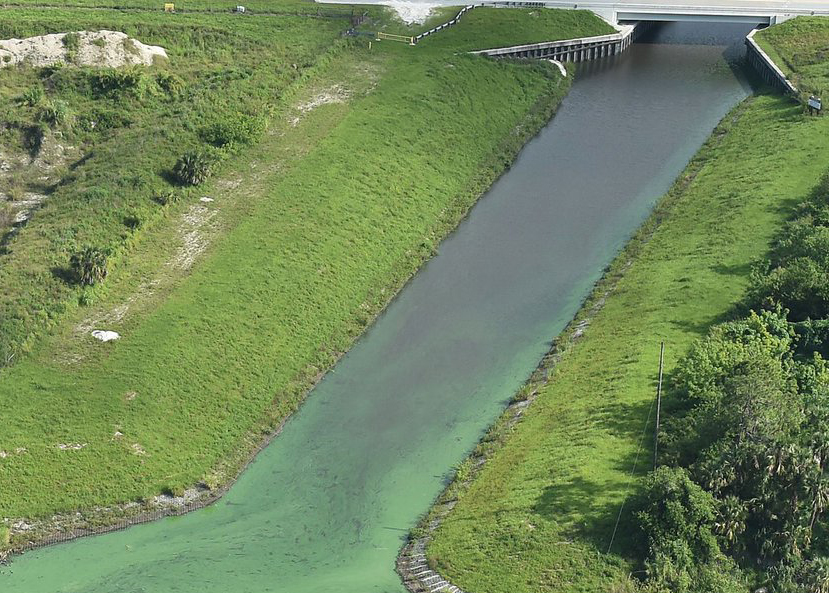
\includegraphics[width=0.5\textwidth]{StLucieCanal.jpg}
    \caption{\textbf{A cyanobacterial bloom in St. Lucie Canal near Indiantown Airport, Florida, on June 8, 2018 (Eric Hasert/TCPalm).} Cyanobacteria density appeared higher near the bank.}
    \label{StLucieCanal}
\end{figure}

We will test 3 different boundary conditions here (\textbf{Figures \ref{CannotSupportPredator}-\ref{PhaseOscillationBlurredByDiffusion}}). In the first scenario, the boundary conditions are set so that the cyanobacteria density cannot support the existence of zooplankton (see part (ii) of the linear stability analysis). As we can see from \textbf{Figures \ref{CannotSupportPredator}}, zooplankton density gradually decreases down the river (more steeply near the bank). In the second scenario, the boundary conditions are set to have a higher total phosphorus concentration (above the supporting threshold of zooplankton) compared to the first scenario, by the addition of extra dissolved phosphorus (from \SI{0.01}{mg/L} to \SI{0.1}{mg/L}). As we can see from \textbf{Figures \ref{ZIncrease}}, zooplankton density indeed increases down the river (again more steeply near the bank).

\begin{figure}[H]
    \centering
    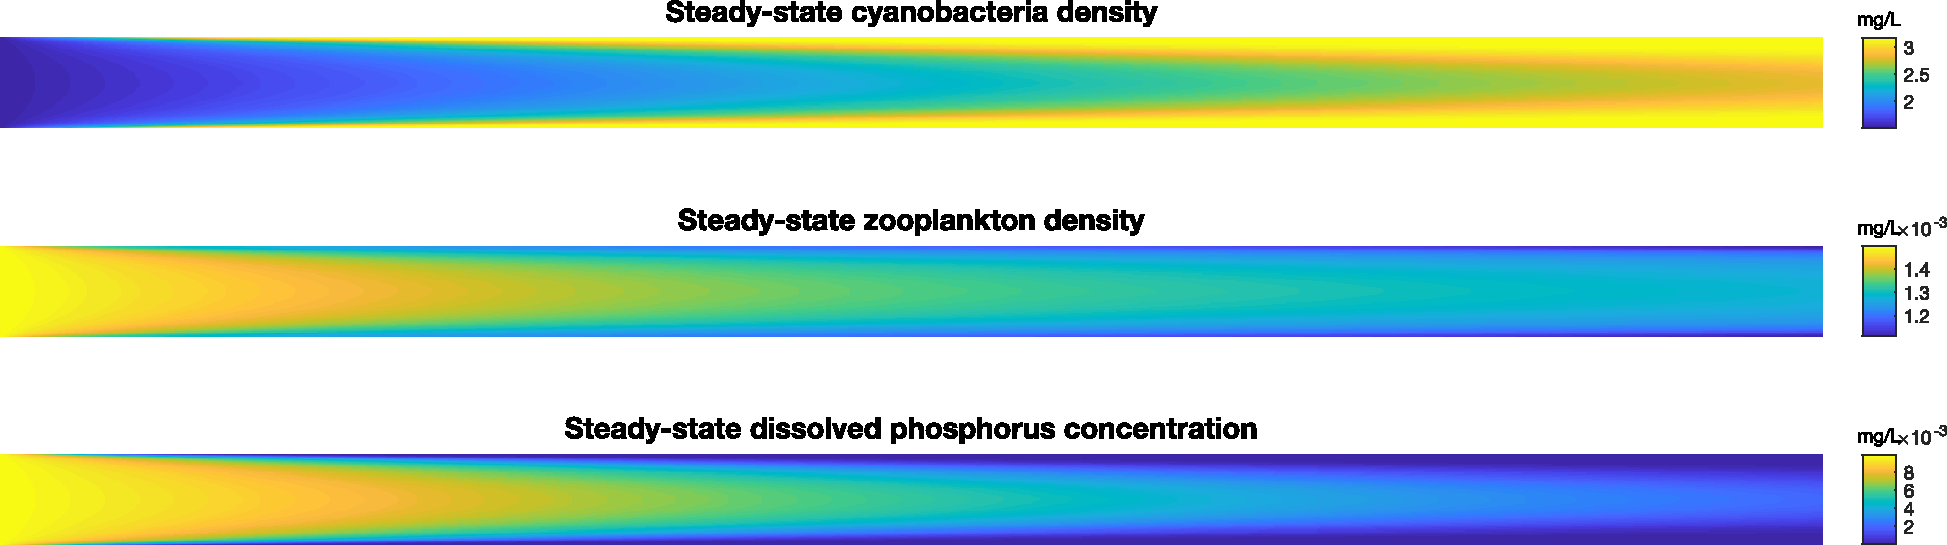
\includegraphics[width=0.95\textwidth]{PreyCannotSupportPredator.pdf}
    \caption{\textbf{Steady-state colormap of the river with boundary conditions that cannot sustain zooplankton along the starting line.} The boundary cyanobacteria density, zooplankton density, and dissolved phosphorus concentration are \SI{1.5}{mg/L}, \SI{0.0015}{mg/L}, and \SI{0.01}{mg/L}, respectively. $v_{\max}$ is set to be \SI{5}{mm/s}.}
    \label{CannotSupportPredator}
\end{figure}

\begin{figure}[H]
    \centering
    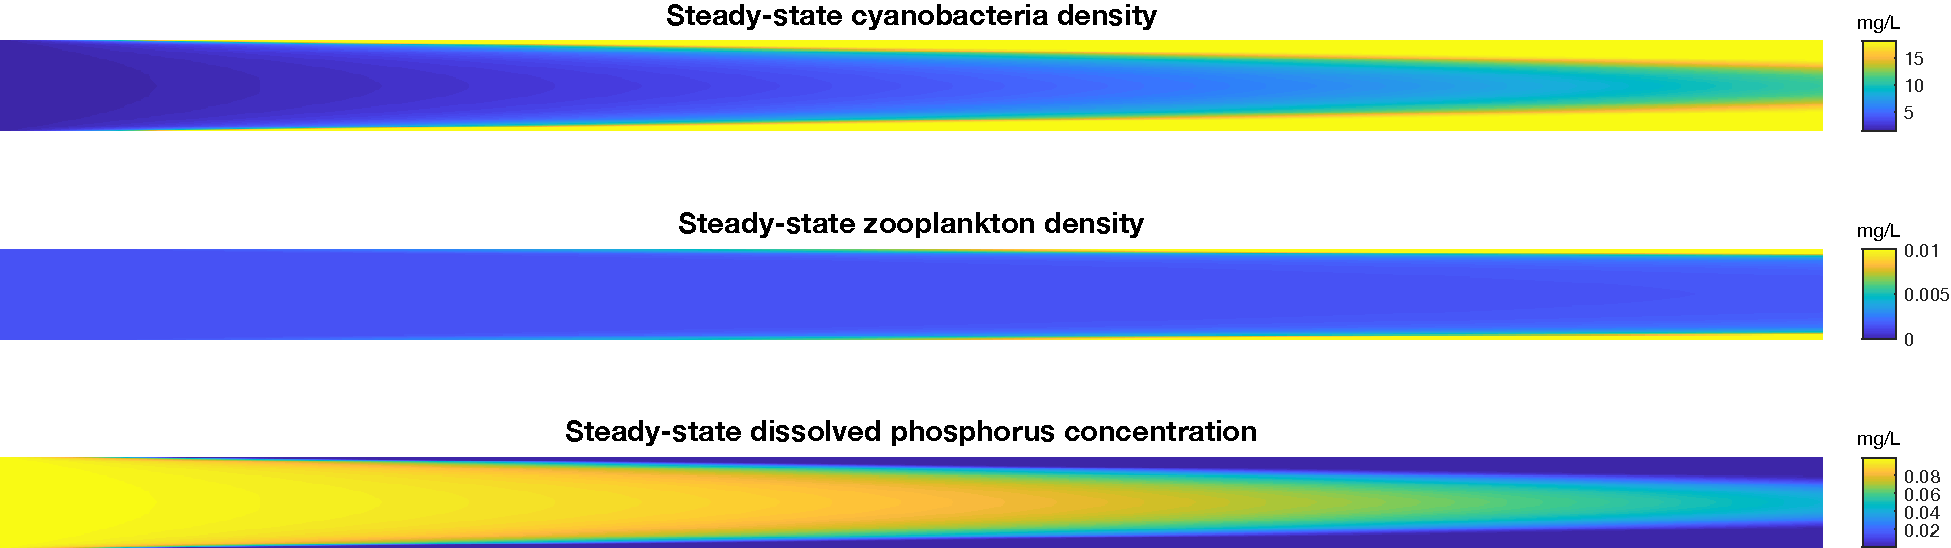
\includegraphics[width=0.95\textwidth]{ZooplanktonIncrease.pdf}
    \caption{\textbf{Steady-state colormap of the river with boundary total phosphorus level above the threshold to sustain zooplankton along the starting line.} The boundary cyanobacteria density, zooplankton density, and dissolved phosphorus concentration are \SI{1.5}{mg/L}, \SI{0.0015}{mg/L}, and \SI{0.1}{mg/L}, respectively. The colorbar of zooplankton density is adjusted and does not cover the entire data range for better visualization. $v_{\max}$ is set to be \SI{5}{mm/s}.}
    \label{ZIncrease}
\end{figure}

The contours are nearly parabolic. This can be explained qualitatively as followed. If we do not consider the diffusion terms (which are actually somewhat insignificant compared to the scale of the river), each streamline (row of the matrix) is independent. We can then define a phase parameter $\phi_{ij} = l_j / v(d_i)$ based on advection. With the boundary conditions that all tiles along the starting line have the same status $(B(0), Z(0), P(0))$, tiles with the same phase $\phi$ should have the same status $(B(\phi), Z(\phi), P(\phi))$. Because the velocity profile is parabolic (equation \ref{v-r}), the patterns naturally resemble parabolas. This also explains the phenomenon that cyanobacteria density is usually higher near the bank of eutrophic, near-quiescent rivers. Water along the bank has a longer retention time in the channel, and cyanobacteria flowing downstream have more time to utilize rich nutrients to proliferate.

In the third scenario, we verify the stability of the non-degenerate fixed point [formula (\ref{Non-trivialFP}); part (iii) of the linear stability analysis]. The boundary status is set to be $(B(0), Z(0), P(0)) = (3.3636, 3.5795, 0.0150)$ mg/L. The rounding errors serve as a tiny disturbance. As shown in \textbf{Figure \ref{PhaseOscillationBlurredByDiffusion}}, the cyanobacteria density, zooplankton density, and dissolved phosphorus concentration are almost homogeneous within the river segment and features phase oscillation (with decreasing amplitudes as phase increases) around the fixed point. 

\begin{figure}[H]
    \centering
    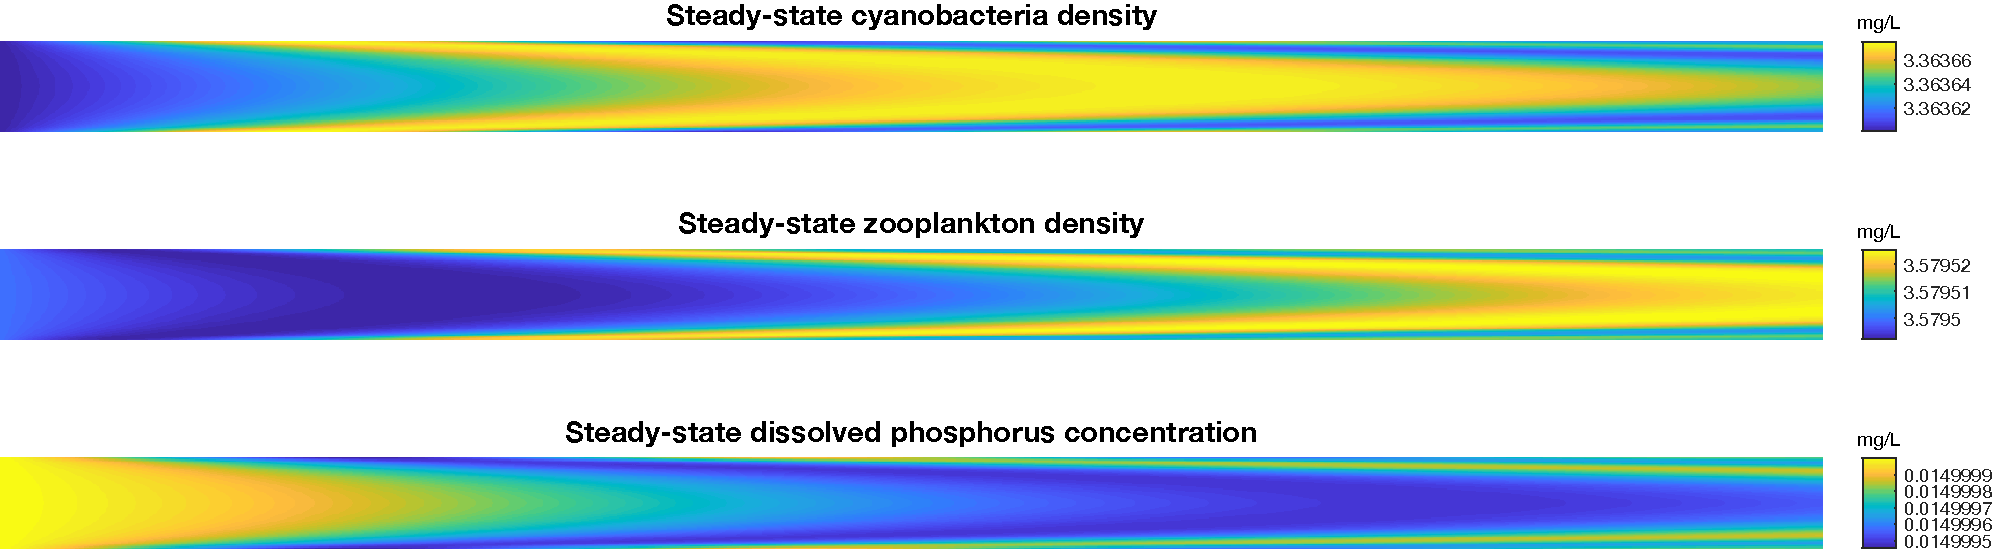
\includegraphics[width=0.95\textwidth]{Point0150Oscillate.pdf}
    \caption{\textbf{Steady-state colormap of the river with boundary conditions set to be at the non-degenerate fixed point along the starting line.} A dissolved phosphorus concentration of \SI{0.0150}{mg/L} is substituted into formula (\ref{Non-trivialFP}), which is below the threshold and therefore corresponds to a stable fixed point according to the linear stability analysis. $v_{\max}$ is set to be \SI{1}{mm/s}.}
    \label{PhaseOscillationBlurredByDiffusion}
\end{figure}

\section*{Discussions}
Other factors may contribute to the aforementioned phenomenon as well.
Near the bank, water is usually warmer in the summer, which facilitates the metabolism and proliferation of cyanobacteria. Irregular bank shapes bays of various sizes, within which water has a long retention time. A realistic non-quiescent water body features chaotic turbulence. The macroscopic consequence of this continuous internal disturbance is the tendency of the system to minimize its mechanical energy. Thus, particles with density higher than that of water appear to be pushed towards slow-flowing regions of the water body. Non-point sources of nutrients (fertilizer runoff and exchange with groundwater \cite{SubsurfaceP}) can also enter the river along the bank or through the bed. Furthermore, the physiology of some cyanobacteria species is reportedly affected by hydrodynamics \cite{HydrodynamicsInfluence}.

This finite-difference modeling framework, together with the Lattice Boltzmann method \cite{BGK} for steady-state flux calculation, should enable cyanobacterial bloom forecast in real lakes based on their precise geometry and inlet/outlet information (locations and discharge). Large freshwater lakes are ecologically and socioeconomically critical, with correlated remote sensing (for quantification of cyanobacteria density \cite{MuPI}), discharge, and water quality data available. In this realistic turbulent environment and at such scale, the model will need to include extra turbulent diffusion terms, while molecular diffusivity and active movement of zooplankton may be ignored depending on the way of discretization.

Previous studies display a large discrepancy on some of the parameter values, which may even vary in the order of magnitude \cite{B}. This hampers reliable modeling studies. Comparing simulations with historic cyanobacterial blooms will help to refine our current model and its parameters, although the algorithm presented here may have to be optimized first to allow for simulations at such scales with reasonable spatial/temporal resolutions.

\printbibliography

\end{document}
